\chapter{Sentiment Analysis}
	Il nostro primo obiettivo è quello di studiare l'intrattenimento, in particolare quali siano i prodotti più recensiti all'interno delle nostre quattro categorie. Come primo passo abbiamo  quindi scelto di effettuare lo studio su un numero limitato di prodotti, riducendoli a duecento, e di analizzare la loro distribuzione. I risultati ottenuti sono presentati nella Figura \ref{fig:pie_category}
		
	\begin{figure} [h]
		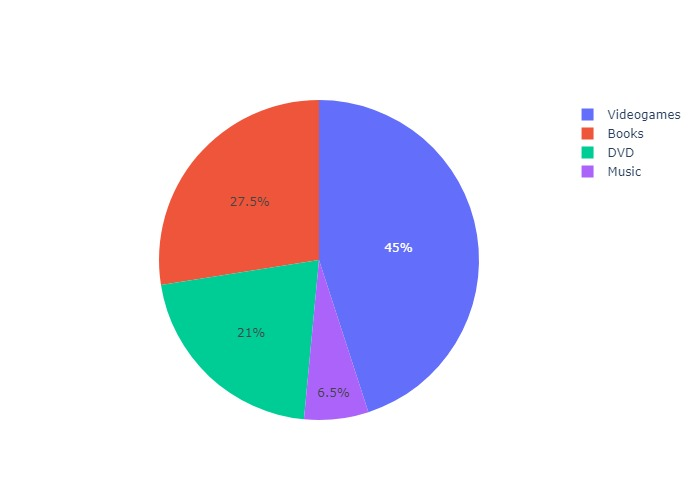
\includegraphics[width=\textwidth]{Figure/pie_category}	
		\caption{Distribuzione delle recensioni per ogni categoria.}
		\label{fig:pie_category}
	\end{figure}
	
	Dalla figura è possibile notare che, in percentuale, i prodotti più recensiti appartengono alla categoria dei videogiochi (\verb|45%|), seguiti dai libri (\verb|27.5%|), dai dvd (\verb|21%|) e dalla musica (\verb|6.5%|). Quest'ultima categoria è davvero esigua perché delle analisi diano risultati consistenti e si possano ricavare informazioni utili; inoltre poiché lo studio su cui abbiamo posto l'attenzione riguardava i più popolari, non aveva senso esaminare dei prodotti quasi privi di recensioni. Da questa considerazione è derivata la scelta di escludere \verb|music| e procedere ad analizzare l'intrattenimento solo sulle tre migliori categorie, quindi \verb|videogames|, \verb|books| e \verb|dvd|. Arrivati a questo punto il nostro studio è stato diviso in due diversi passaggi, durante i quali abbiamo cercato di rispondere a due domande ovvero quali siano i prodotti più recensiti e perché proprio loro. 
		
	\section{Primo passaggio: distribuzione del sentiment}
		Come già accennato, per poter valutare la polarità di una recensione è necessario calcolare il \textit{sentiment}. Abbiamo visto che questo calcolo può essere eseguito secondo diverse metodologie, tuttavia il nostro \textit{dataset} relativo ai prodotti, presentava al suo interno un campo che ben si prestava a questo tipo di analisi. L'attributo in questione è quello delle stelle. \textit{Amazon} infatti per ogni recensione riferita a un determinato prodotto associa una valutazione in stelle da \verb|0| a \verb|5|. Questo ha permesso di effettuare un conteggio per ogni prodotto di tutte le sue recensioni, dividendole in positive negative e neutre, secondo lo schema di seguito.
			
		\begin{itemize}
			\item \textbf{positive:} la recensione aveva un punteggio di maggiore di tre stelle.
			\item \textbf{neuter:} la recensione aveva un punteggio uguale a tre stelle.
			\item \textbf{negative:} la recensione aveva un punteggio minore di tre stelle.
		\end{itemize}
			
		Procedendo secondo queste modalità, preso per esempio il prodotto "Zelda", con \verb|200| recensioni, si calcolano quante di queste sono risultate positive negative oppure neutre e un possibile risultato potrebbe essere costituito da \verb|100| recensioni positive, \verb|70| negative e \verb|30| neutre. \\		
		Ottenuto questo elenco abbiamo calcolato la distribuzione probabilistica associata alle tre diverse polarità. In particolare per ognuna associata a uno specifico prodotto, abbiamo effettuato un rapporto tra il conteggio delle recensioni positive e negative, escludendo le neutre (dato non rilevante per la nostra analisi) e il numero di recensioni totali. 
			
		La distribuzione probabilistica della polarità ottenuta è stata quindi combinata al sottoinsieme dei prodotti più recensiti/più popolari e il risultato di questo \textit{match} è stata l'identificazione per ogni categoria dei primi cinque prodotti più popolari suddivisi in due elenchi. Il primo contenente i prodotti valutati più negativamente e nel secondo quelli valutati più positivamente. \\
		I risultati ottenuti sono visibili nelle Figure \ref{fig:top_pos_book_table} \ref{fig:top_neg_book_table}, \ref{fig:top_pos_film_table}, \ref{fig:top_neg_film_table}, \ref{fig:top_pos_videogames_table}, \ref{fig:top_neg_videogames_table}.
			
		\begin{figure} [h]
			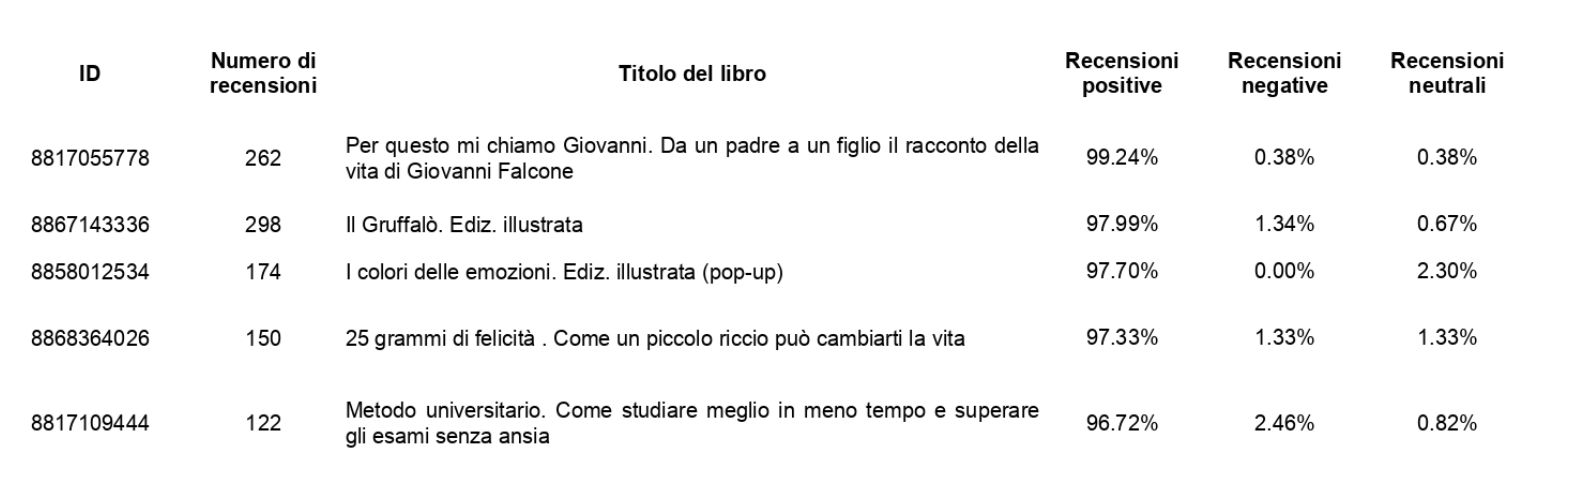
\includegraphics[width=\textwidth]{Figure/top_pos_book_table}
			\caption{Primi cinque libri con più recensioni positive}
			\label{fig:top_pos_book_table}
		\end{figure}
			
		\begin{figure} [h]
			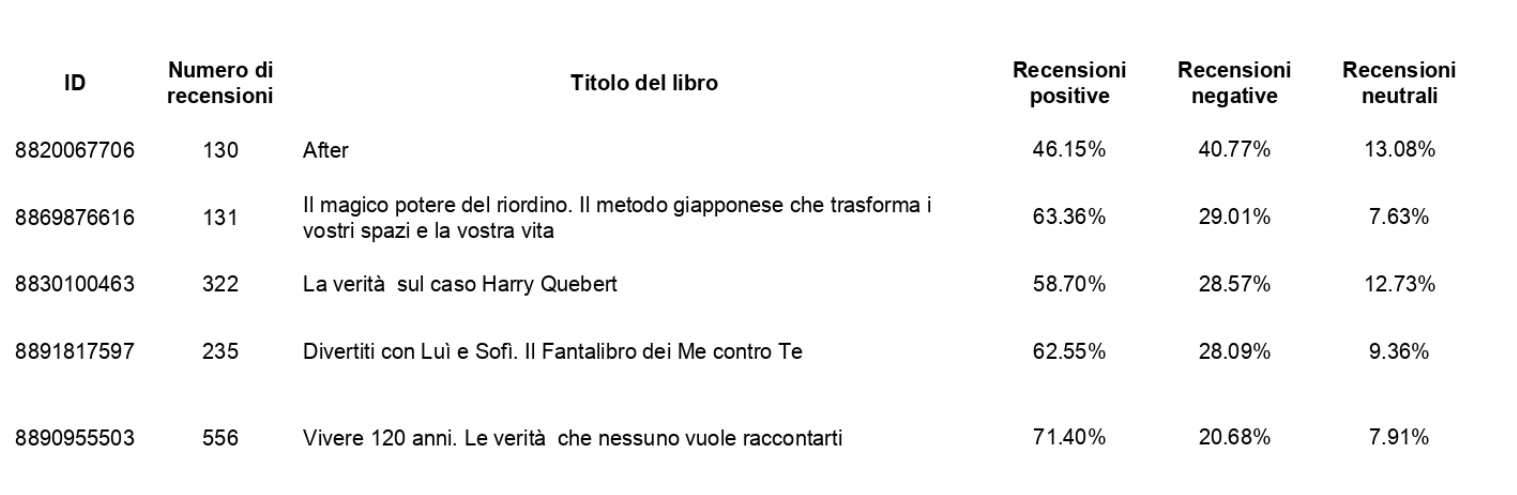
\includegraphics[width=\textwidth]{Figure/top_neg_book_table}
			\caption{Primi cinque libri con più recensioni negative}
			\label{fig:top_neg_book_table}
		\end{figure}
		
		\begin{figure} [h]
			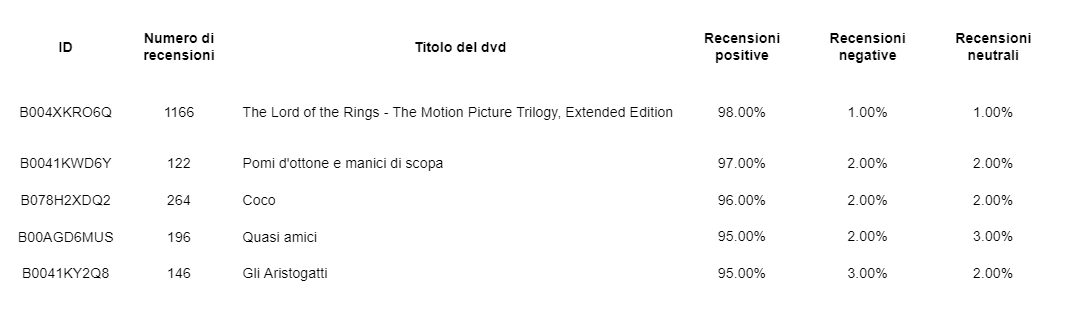
\includegraphics[width=\textwidth]{Figure/top_pos_film_table}
			\caption{Primi cinque dvd con più recensioni positive}
			\label{fig:top_pos_film_table}
		\end{figure}
		
		\begin{figure} [h]
			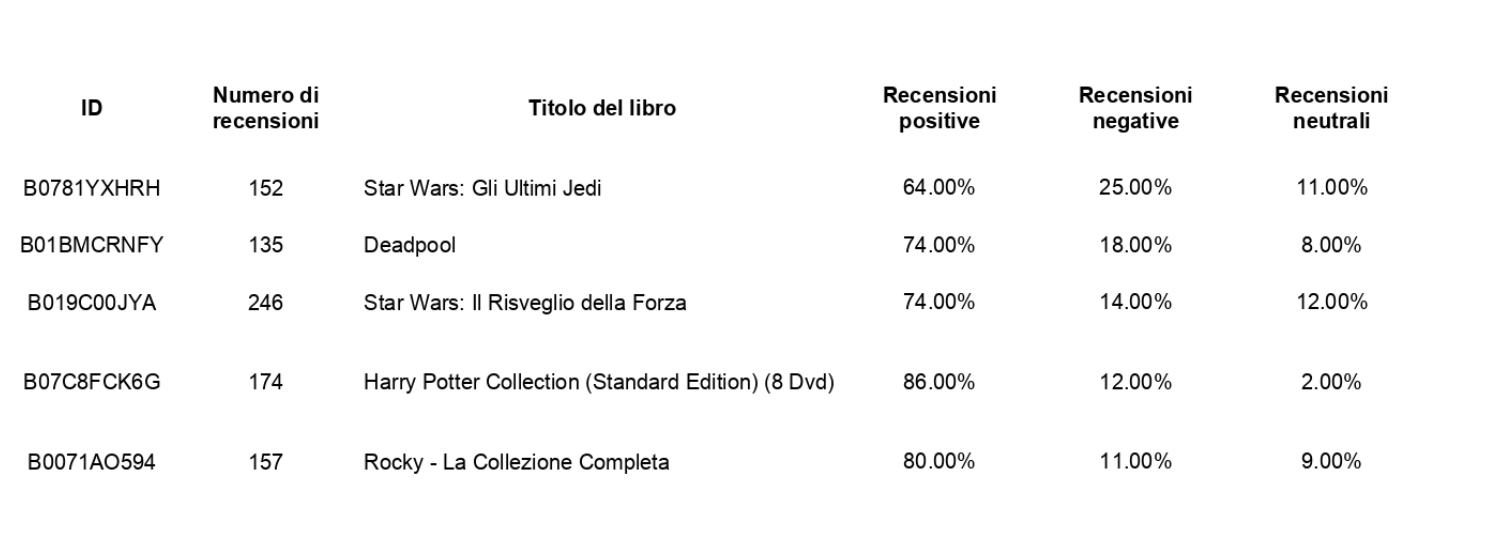
\includegraphics[width=\textwidth]{Figure/top_neg_film_table}
			\caption{Primi cinque dvd con più recensioni negative}
			\label{fig:top_neg_film_table}
		\end{figure}
		
		\begin{figure} [h]
			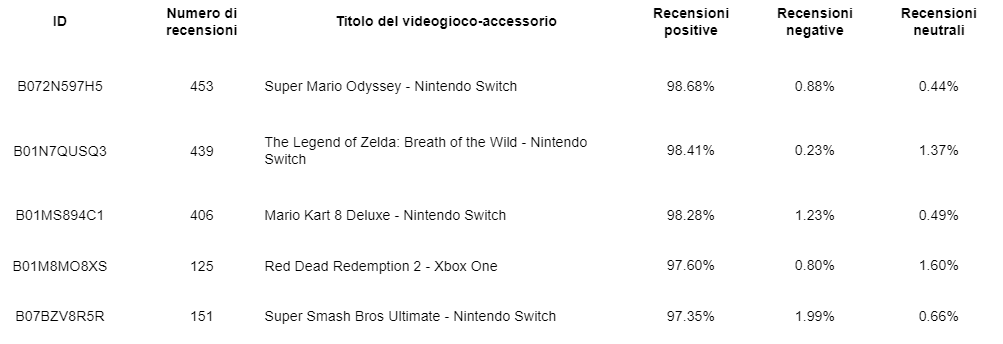
\includegraphics[width=\textwidth]{Figure/top_pos_videogames_table}
			\caption{Primi cinque videogiochi con più recensioni positive}
			\label{fig:top_pos_videogames_table}
		\end{figure}
		
		\begin{figure} [h]
			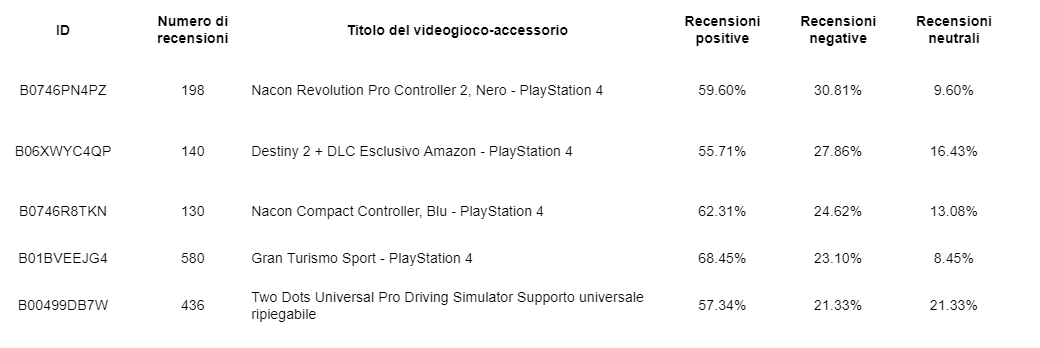
\includegraphics[width=\textwidth]{Figure/top_neg_videogames_table}
			\caption{Primi cinque videogiochi con più recensioni negative}
			\label{fig:top_neg_videogames_table}
		\end{figure}
		
	
	\section{Secondo passaggio: analisi delle parole più usate}
		Avendo risposto al primo quesito ci siamo potuti soffermare sulla seconda interrogazione, ovvero perché fossero risultati proprio questi prodotti. Siamo così andati alla ricerca delle parole più utilizzate all'interno delle recensioni (negative e positive), cercando una corrispondenza tra queste e i prodotti migliori. Tuttavia per poter eseguire questo confronto sono state necessarie delle operazioni atte a uniformare il \textit{dataset}; i dati infatti non sempre sono puliti, in essi sono presenti errori di battitura, intere frasi scritte in maiuscolo, eccessiva punteggiatura, etc. Ecco dunque il motivo del termine "uniformare", intendiamo con esso il processo di riscrittura delle frasi seguendo degli specifici passaggi, che saranno descritti nel seguito.
			
		\begin{description}
			\item[tokenizzazione:] suddivide un testo in singole parole, i\textit{token}), che saranno utilizzati per altri tipi di analisi o attività.
			\item[standardizzazione:] riscrittura delle parole da \textit{upper case} a \textit{lower case}. 
			\item[rimozione delle \textit{stopwords},] parole comuni prive di significato, ma che ricorrono spesso all'interno della frasi.
			\item[rimozione delle cifre numeriche]
			\item[rimozione della punteggiatura,] tuttavia nella nostra implementazione questa fase è subentrata all'interno della \verb|tokenizzazione|. 
			\item [stemming:] processo di riduzione delle parole flesse (o talvolta derivate) alla loro forma di origine, base o radice.
		\end{description}
			
		Al termine del processo, l'\textit{output} risultante era composto da un elenco di parole scritte Italiano corretto, privo di segni di punteggiatura o numeri, scritto in forma minuscola, ridotto alla radice. A questo punto è stato quindi possibile effettuare un'operazione di visualizzazioni delle parole più usate all'interno delle recensioni, per comprendere il motivo per cui proprio quei prodotti presenti nella lista rientrino nei migliori, per entrambe le polarità. La tecnica visiva utilizzata è quella dei \verb|wordclouds|, che consiste nella raccolta delle parole più usate nelle recensioni (\verb|word|), rappresentate per mezzo di \verb|cloud|, ha permesso di confrontare le recensioni positive e negative per ogni categoria e di comprendere che cosa determinava l'appartenenza dei prodotti all'insieme dei "migliori" o dei peggiori. 
		
		\subsection{Wordclouds libri} ????????????????????????? manca corrispondenza tabella
			Nella Figura \ref{fig:wordclouds_book} sono mostrati i \textit{wordclouds} ottenuti per la categoria libri. In particolare l'immagine di sinistra rappresenta le parole più usate nelle recensioni positive, mentre a destra sono rappresentate quelle negative. 
			
			\begin{figure} [h]
				\centering
				\begin{subfigure}{0.48\textwidth}
					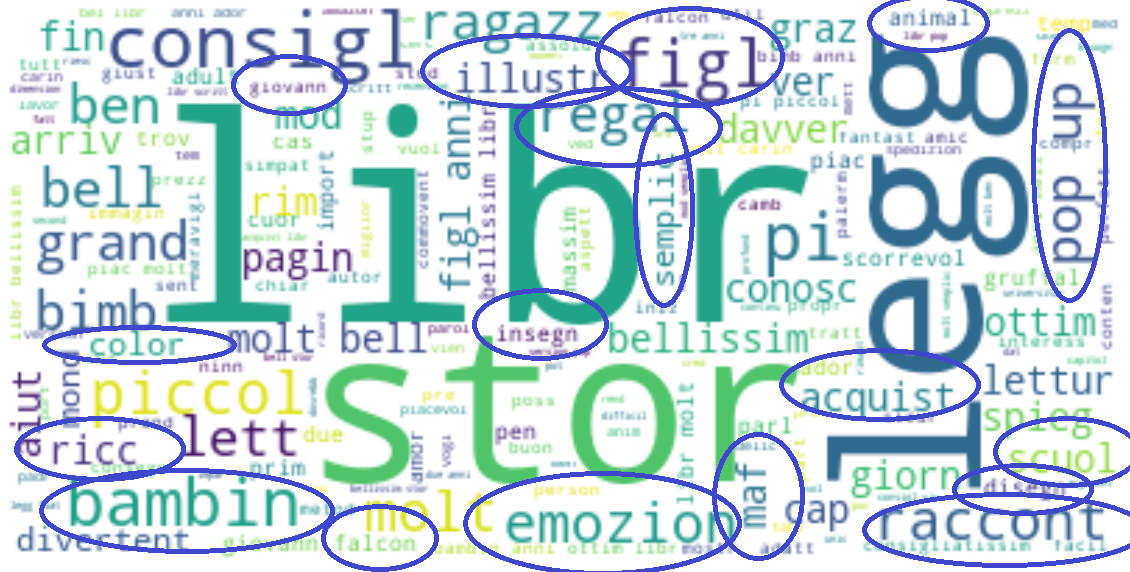
\includegraphics[width=\textwidth]{Figure/top_positive_books}
					\caption{Recensioni positive}
					\label{fig:top_positive_books}
				\end{subfigure}
				\begin{subfigure}{0.48\textwidth}
					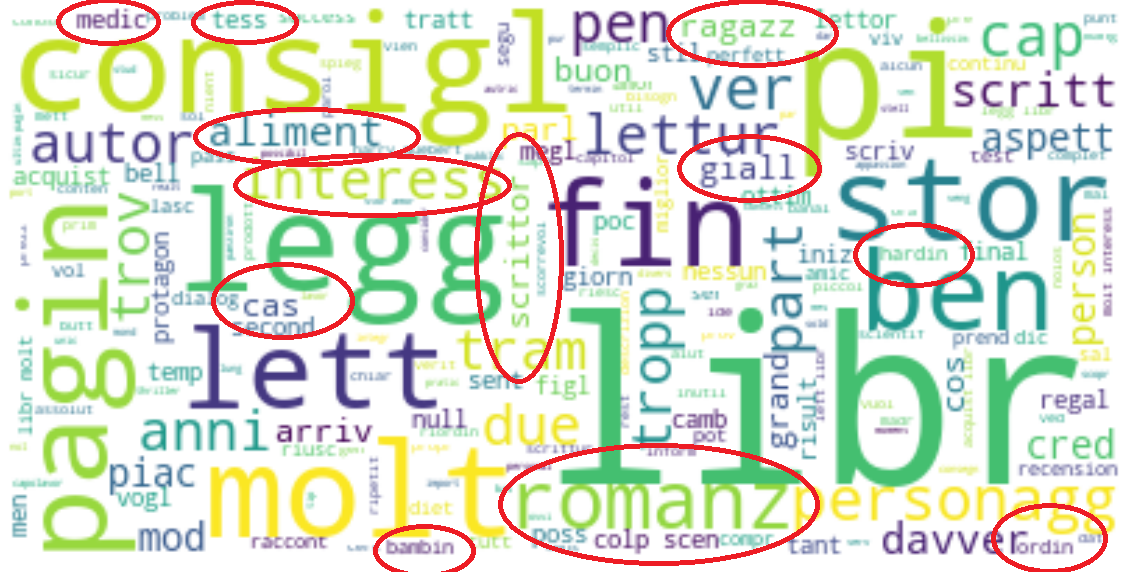
\includegraphics[width=\textwidth]{Figure/top_negative_books}
					\caption{Recensioni negative}
					\label{fig:top_negative_books}
				\end{subfigure}
				\caption{Wordclouds libri}\label{fig:wordclouds_book}
			\end{figure}
			
			\begin{description}
				\item[Recensioni positive:]
				 nello schema sono rappresentate con dimensione maggiore le parole \verb|libr|, \verb|stori|, \verb|legg|, a dimostrazione del fatto che queste sono in assoluto le parole più frequenti all'interno delle recensioni degli utenti. Non sorprende che i tre termini si riferiscano alla categoria selezionata, nel caso attuale quella dei libri; vedremo che questo comportamento ricorrerà spesso nell'analisi sui \textit{wordclouds}. Concentriamoci invece sulle parole che racchiudono informazioni. 	
				\begin{itemize}
					\item \texttt{illustr}, \texttt{bambin}, \texttt{color}, \texttt{semplic},  \texttt{disegn}, \texttt{raccont}, \texttt{animal} : \\
					sono tutti termini riguardanti l'infanzia. Da questa informazioni comprendiamo che la maggior parte delle recensioni commenta positivamente i libri per bambini, che sono semplici, colorati, ricchi di disegni e di racconti basati sugli animali. 
					\item \texttt{regal}: \\
					molto probabilmente alcuni libri, comprati per un regalo, hanno suscitato delle impressioni positive nell'utente, che ha quindi recensito positivamente.
				\end{itemize}	
			
				\item[Recensioni negative:] 
				nello schema sono rappresentate con dimensione maggiore le parole \verb|libr|, \verb|pagin|, \verb|legg|, a dimostrazione del fatto che queste sono in assoluto le parole più frequenti all'interno delle recensioni degli utenti. Notiamo che due su tre sono parole già trovate all'interno dell'elenco delle parole positive, poiché anche in questo caso sono termini utili a determinare la categoria in questione.
				\begin{itemize}
					\item \texttt{medic}, \texttt{romanz}, \texttt{giall}, \texttt{aliment} : \\
					sono tutti termini riguardanti i possibili generi di un libro. L'informazione che ricaviamo è che i libri riguardanti la medicina, la cucina, i gialli e i romanzi, sono quelli che più di tutti sono stati criticati.			
				\end{itemize}
			\end{description}
		
		
		\subsection{Wordclouds dvd}
			Nella Figura \ref{fig:wordclouds_dvd} sono mostrati i \textit{wordclouds} ottenuti per la categoria dvd. In particolare l'immagine di sinistra rappresenta le parole più usate nelle recensioni positive, mentre a destra sono rappresentate quelle negative. 
				
			\begin{figure} [h]
				\centering
				\begin{subfigure}{0.48\textwidth}
					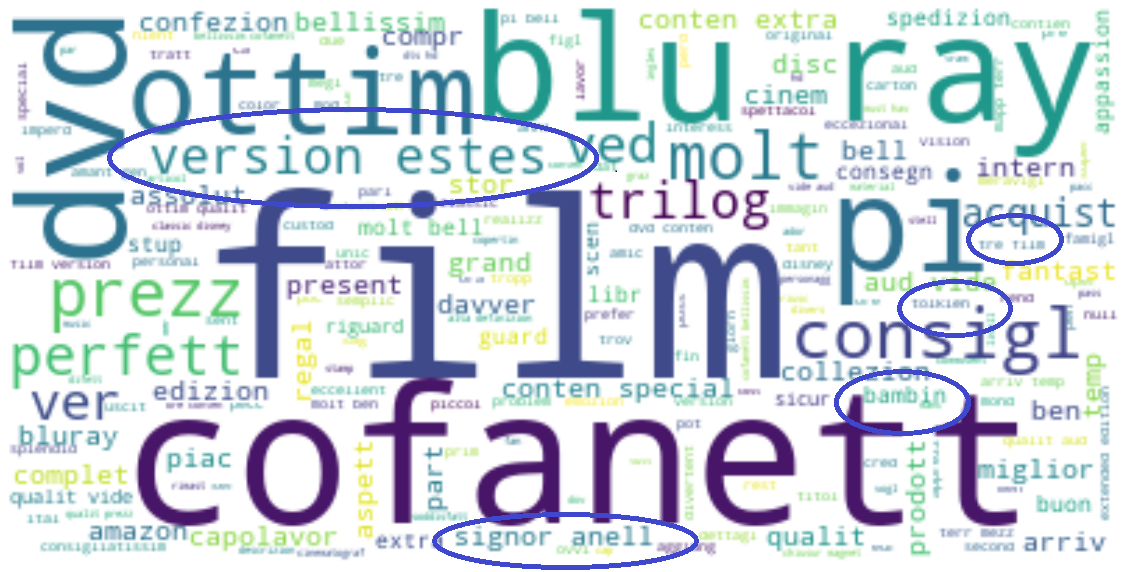
\includegraphics[width=\textwidth]{Figure/top_positive_dvd}
					\caption{Recensioni positive}
					\label{fig:top_positive_dvd}
				\end{subfigure}
				\begin{subfigure}{0.48\textwidth}
					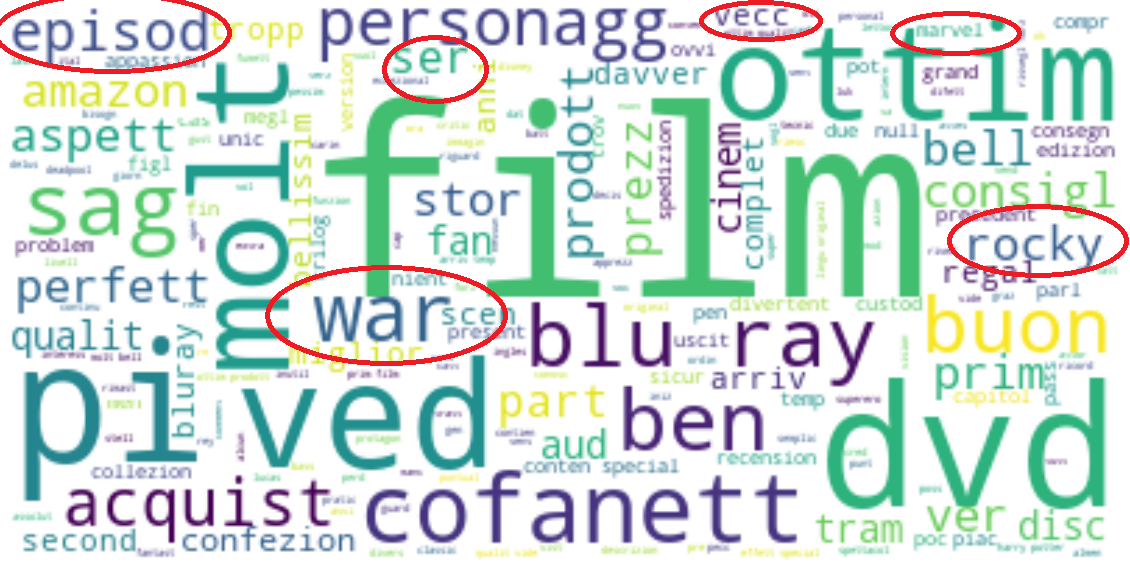
\includegraphics[width=\textwidth]{Figure/top_negative_dvd}
					\caption{Recensioni negative}
					\label{fig:top_negative_dvd}
				\end{subfigure}
				\caption{Wordclouds dvd}\label{fig:wordclouds_dvd}
			\end{figure}
		
				\begin{description}
				\item[Recensioni positive:]
				nello schema sono rappresentate con dimensione maggiore le parole \verb|dvd|, \verb|film|, \verb|blu ray|, riferite genericamente alla categoria presa in esame. 	
				\begin{itemize}
					\item \texttt{signore anell}, \texttt{tolkien}, \texttt{tre film}: \\
					I termini selezionati sono accomunati dalla tematica "Signore degli Anelli", trilogia ispirato all'omonimo romanzo scritto da Tolkien, che ha raccolto molti consensi, dato che più parole lo caratterizzano.
					\item \texttt{bambin}: \\
					I dvd criticati positivamente sono stati quelli adatti a un giovane pubblico. Da notare che il termine risponde ancora alle caratteristiche del "Signore degli Anelli".
					\item \texttt{version estes}: \\
					Tra i tanti comprati o visti, i dvd in versione estesa hanno riscontrato un consenso positivo.
				\end{itemize}	
			
				Si noti che le parole trovate ben si accordano con i risultati trovati nei passaggi precedenti (Figura \ref{fig:top_pos_film_table}), dove il miglior prodotto era la trilogia del "Signore degli anelli", seguito poi da altri film adatti ai bambini ("Coco", terzo posto, e "Gli Aristogatti", sono addirittura dei cartoni animati).
				
				\item[Recensioni negative:] 
				nello schema i termini generici riscontrabile con la categoria in questione sono \verb|film|, \verb|dvd |, \verb|blu ray|. Poiché nella Figura \ref{fig:top_neg_film_table}, abbiamo trovato cinque prodotti di diversa natura come maggiormente criticati, ci aspettiamo di trovare termini che li identifichino e che argomentino le recensioni negative.
				\begin{itemize}
					\item \texttt{war}, \texttt{marvel}, \texttt{rocky}: \\
					sono tutti termini utili a identificare il dvd in questione. Come ci aspettavamo, il primo di questi si riferisce al film di "Star Wars", il primo peggio criticato, il secondo invece riguarda "Deadpool", un film della marvel e il terzo del film "Rocky". 
					\item \texttt{ser}, \texttt{episod}, \texttt{vecc}: \\
					In queste parole sono racchiuse le cause delle critiche. I primi due probabilmente rivolti a "Star Wars", una serie di nove film, ognuno dei quali denominato con il termine di "episodio". Il terzo vocabolo, che molto probabilmente si rifesce a "Rocky", criticato invece per l'età.		
				\end{itemize}
			\end{description}
		
		